\subsection{Lab9: Transmisor FM monofónico}

%*********************
\begin{frame}{}

\pgfdeclareimage[width=\paperwidth,height=\paperheight]{bg}{imagenes/fondo_lab}
\setbeamertemplate{background}{\pgfuseimage{bg}}

\bfseries{\textrm{\LARGE Lab9\\ \Large Transmisor FM monofónico}}
\raggedright
\end{frame}
%*********************

\begin{frame}{Transmisor FM monofónico}

\pgfdeclareimage[width=\paperwidth,height=\paperheight]{bg}{imagenes/fondo3}
\setbeamertemplate{background}{\pgfuseimage{bg}}

El transmisor FM monofónico es un dispositivo electrónico que, mediante una antena, irradia ondas electromagnéticas que contienen (o pueden contener) información, como ocurre en el caso de las señales de radio.\\ \vspace{2mm}
Por medio de la modulación angular se puede hacer que un parámetro de la onda portadora cambie de valor según las variaciones de la señal moduladora, que es la información que queremos transmitir. \\ \vspace{2mm}
Se utiliza esta modulación porque facilita la propagación de la señal de información, ordena el radio espectro, disminuye dimensiones de antenas, optimiza el ancho de banda de cada canal, evita interferencias entre canales y protege la información de las degradaciones por ruido.



\end{frame}
%---------------------------------
\begin{frame}{Transmisor FM monofónico}

\begin{figure}[H]
\centering
\vspace{-3mm}
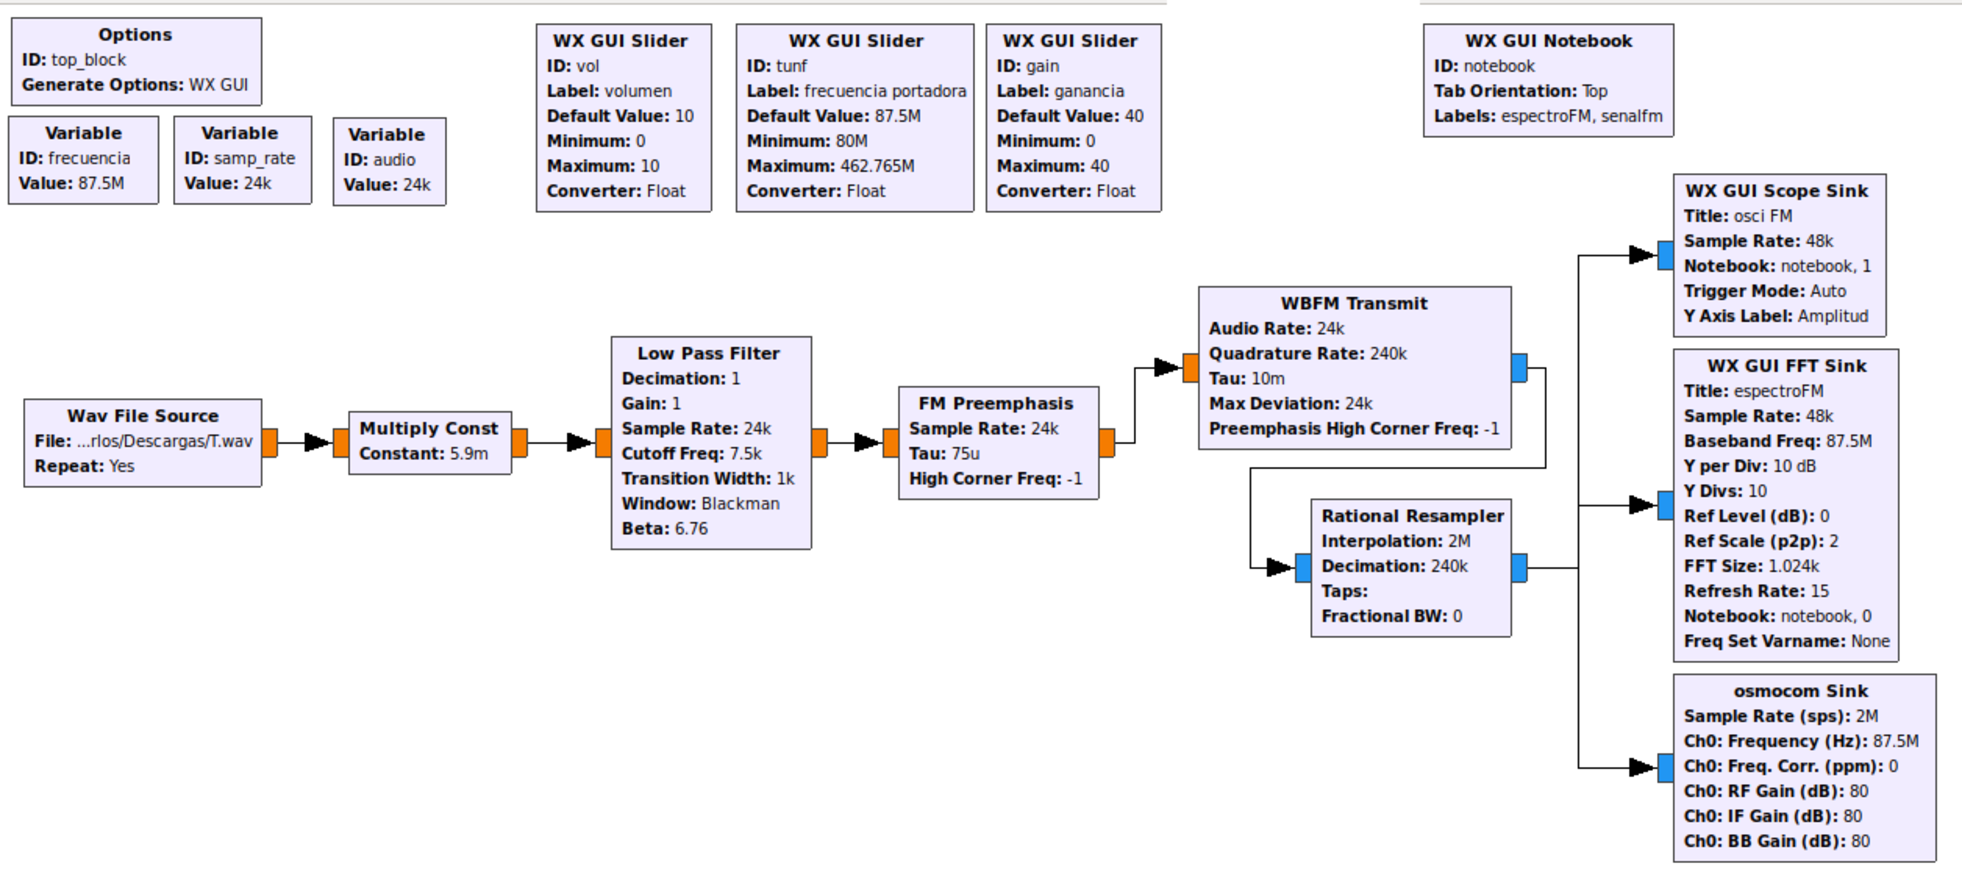
\includegraphics[width=\textwidth]{parte3/lab11/pdf/lab11_1.pdf}
\end{figure}

\end{frame}
%---------------------------------

\begin{frame}{Transmisor FM monofónico}

\begin{figure}[H]
\centering
\vspace{-3mm}
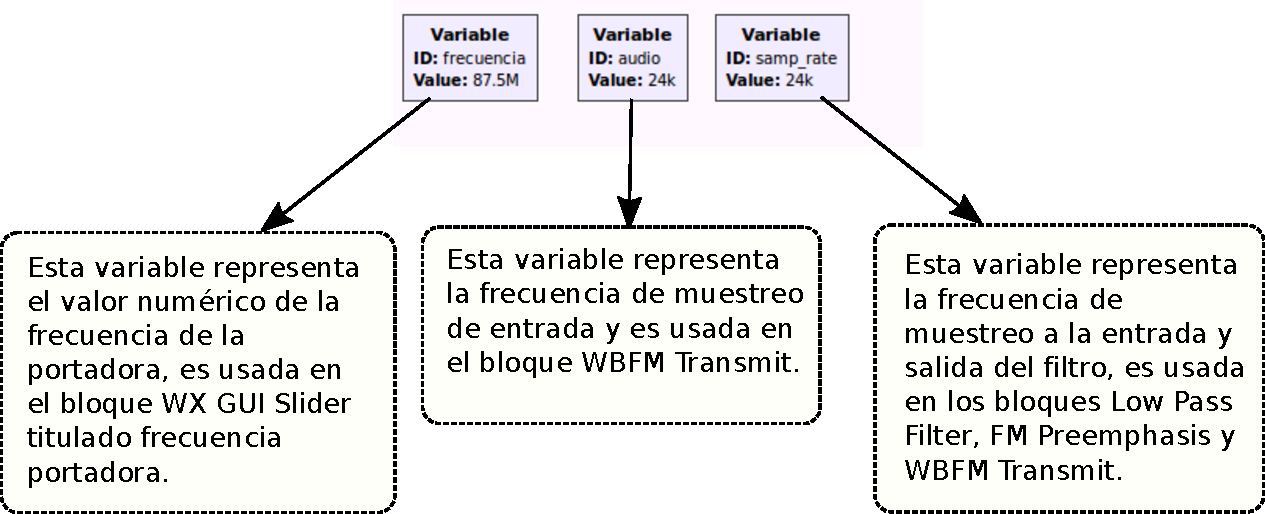
\includegraphics[width=\textwidth]{parte3/lab11/pdf/lab11_2.pdf}
\end{figure}


\end{frame}
%---------------------------------

\begin{frame}{Transmisor FM monofónico}

\begin{figure}[H]
\centering
\vspace{-3mm}
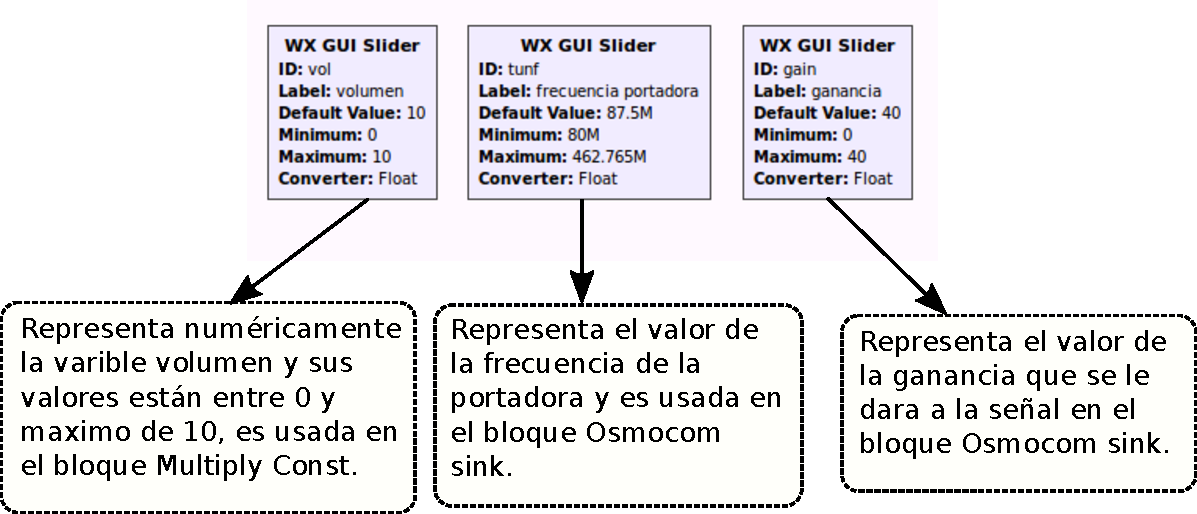
\includegraphics[width=\textwidth]{parte3/lab11/pdf/lab11_3.pdf}
\end{figure}

\end{frame}
%---------------------------------

\begin{frame}{Transmisor FM monofónico}

\begin{figure}[H]
\centering
\vspace{-3mm}
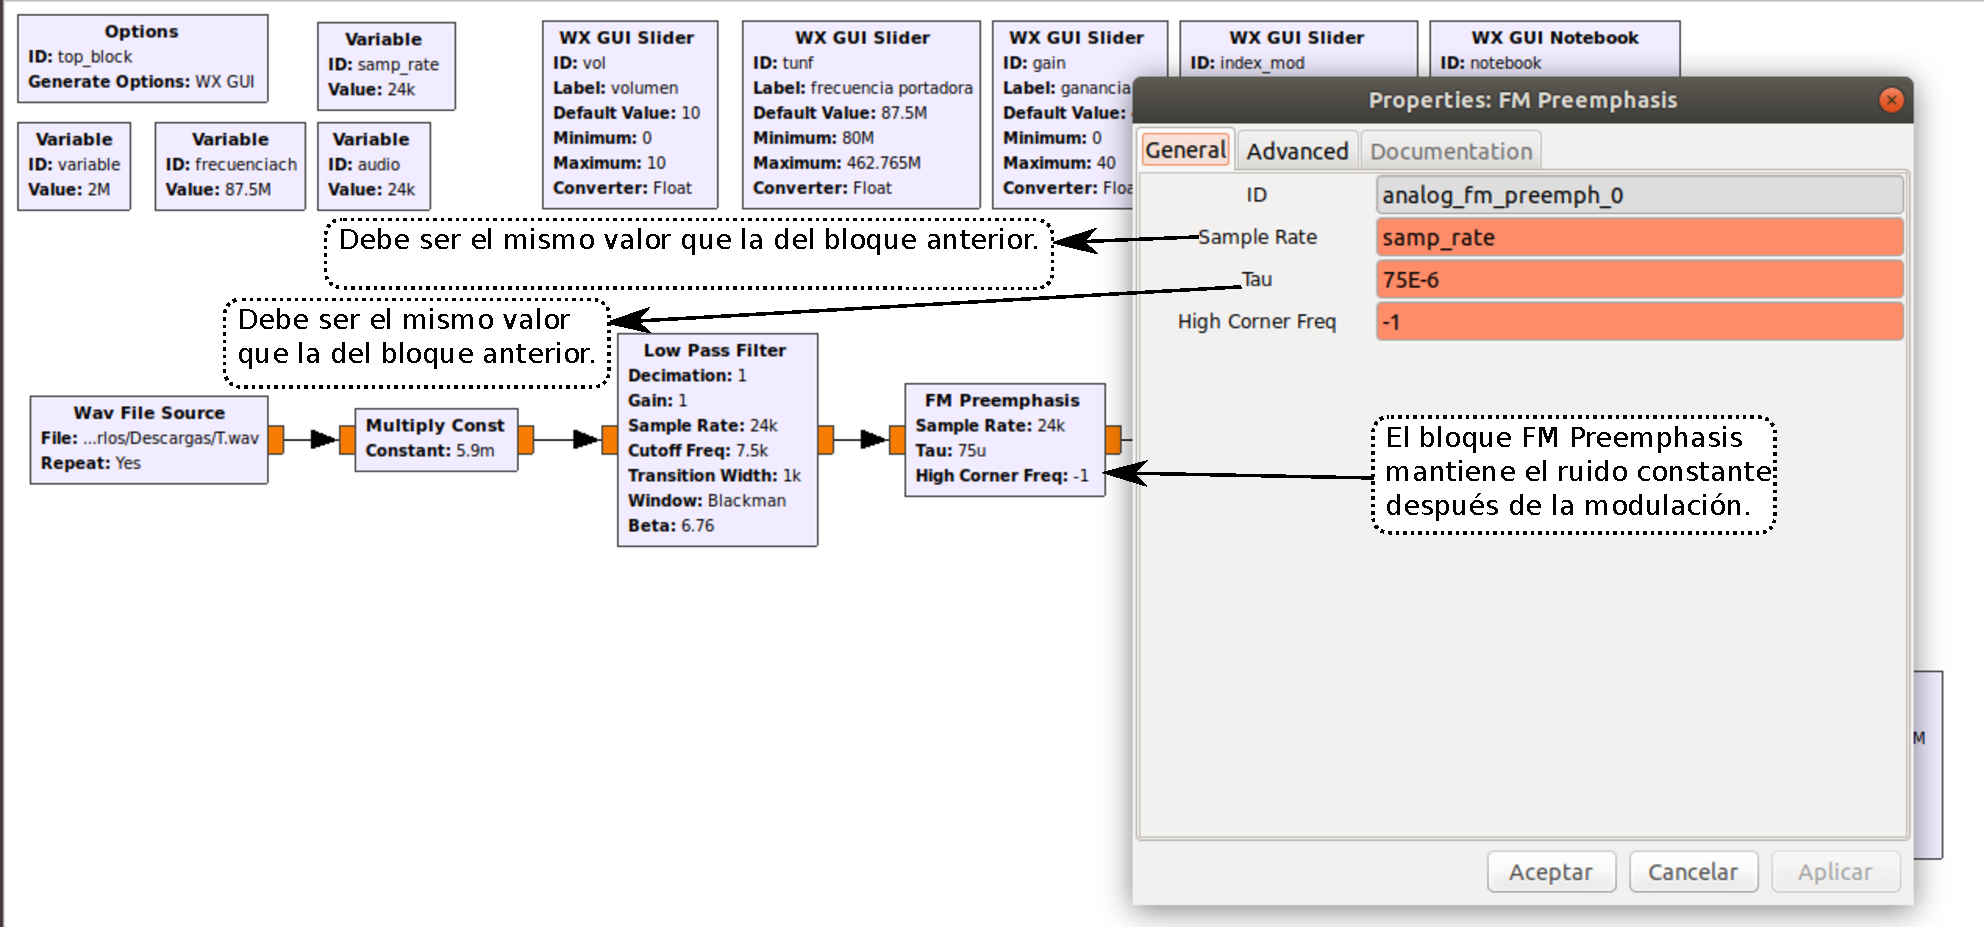
\includegraphics[width=\textwidth]{parte3/lab11/pdf/lab11_4.pdf}
\end{figure}

En este transmisor FM monofónico la fuente es un archivo de audio en formato WAV muestreado a 24 kHz.  

\end{frame}
%---------------------------------

\begin{frame}{Transmisor FM monofónico}

Mediante el uso de la orden \texttt{file} en la consola, se puede consultar la frecuencia de muestreo de un archivo de audio de la siguiente forma (en este caso formato WAV).

\begin{itemize}
    \item {Ingresando a la consola y mediante la opción \texttt{cd} buscar la carpeta donde está ubicado el archivo de audio.}
    \item {Una vez ubicado en la carpeta desde el terminal con la opción \texttt{ls} se pueden ver los nombres de archivos que se alojan en esa ubicación, de esta forma se verá el nombre del archivo de audio.}
    \item {Con el nombre del archivo de audio, usar \texttt{file} de la siguiente manera:  
}
    \begin{block}{}
    \texttt{
    \ \ \ file + nombre del archivo.wav}
    \end{block}
    
\end{itemize}{}

\end{frame}
%---------------------------------

\begin{frame}{Transmisor FM monofónico}

Si la frecuencia de muestreo de un archivo de audio se desea cambiar es posible hacerlo mediante el uso de la orden \texttt{sox} así:

\begin{itemize}
    \item {Con la ubicación y el nombre del archivo de audio de formato WAV usar \texttt{sox}.}
    \item {Como ejemplo, para un archivo que se llame \textbf{“audio1.wav”} y que esté muestreado a 44100 Hz y se requiera cambiar a 24000 Hz se usaría la orden así:
     \begin{block}{}
    \texttt{
    \ \ \ sox audio1.wav -r 24000 audio2.wav  }
    \end{block}}
    \item {El nombre se cambia al final ya que lo que se hace es crear un nuevo archivo de audio con una frecuencia de muestreado diferente.  
}
   
    
\end{itemize}{}

\end{frame}
%---------------------------------

\begin{frame}{Transmisor FM monofónico}

\begin{figure}[H]
\centering
\vspace{-3mm}
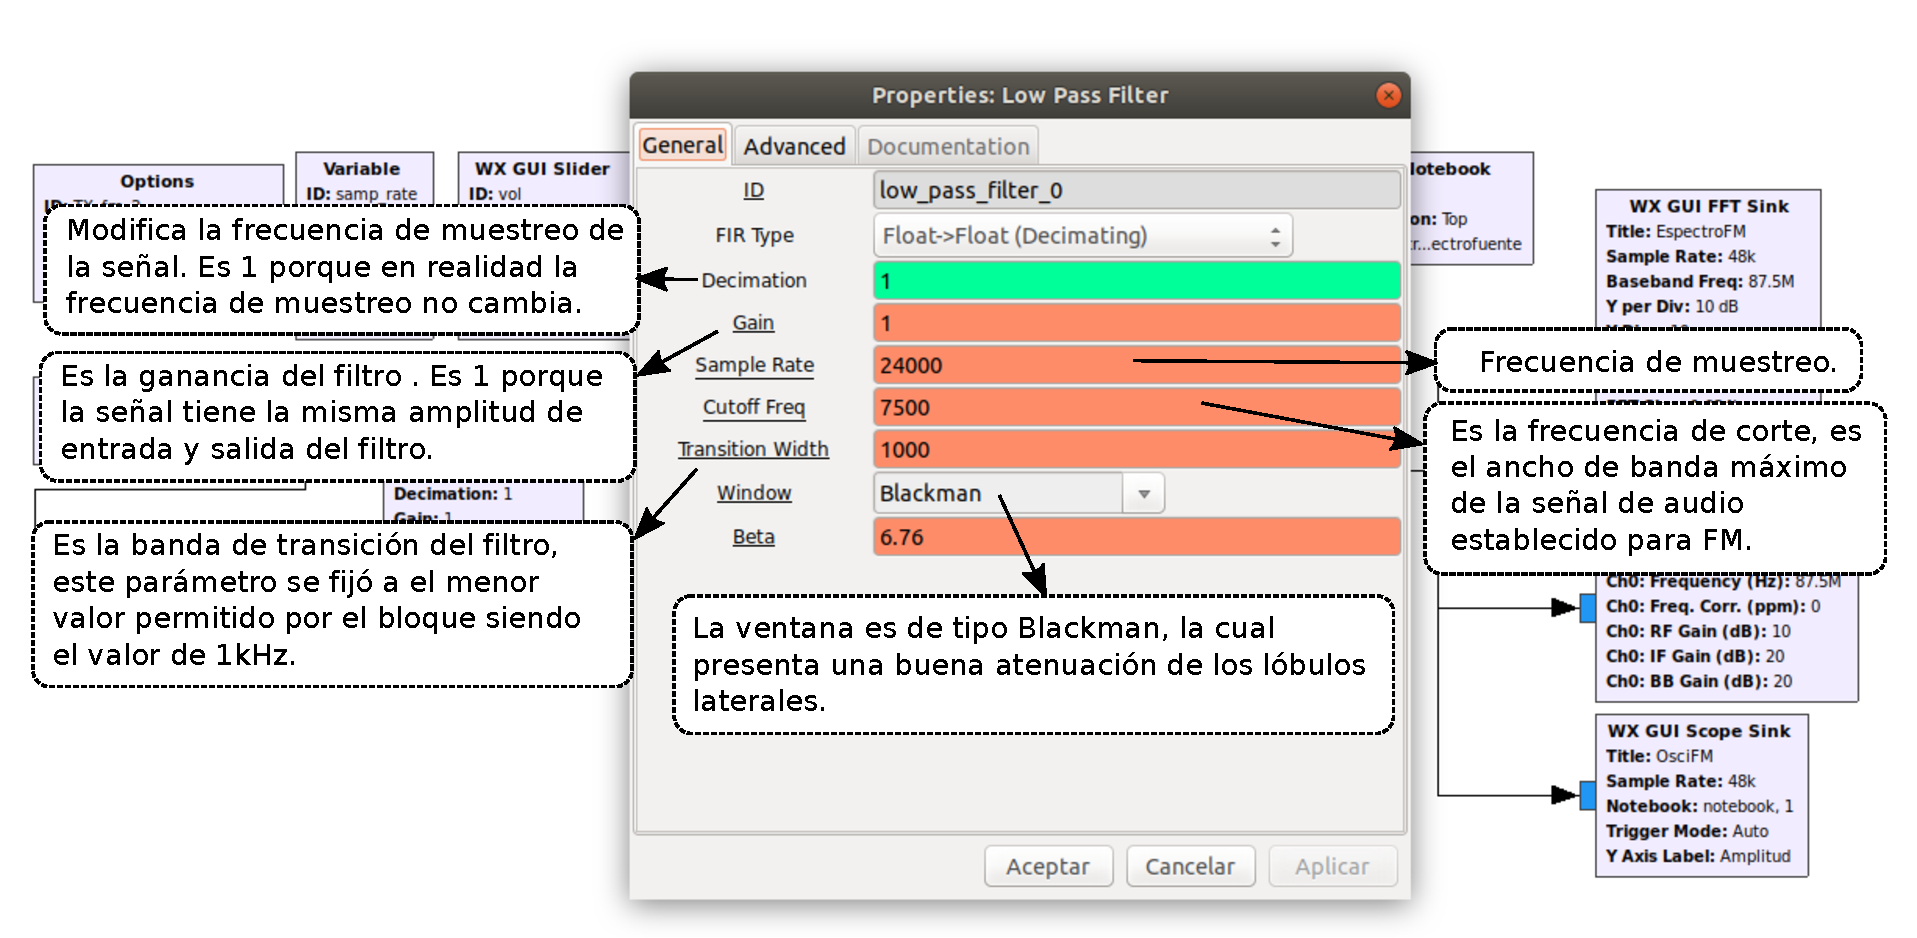
\includegraphics[width=1.1\textwidth]{parte3/lab11/pdf/lab11_5.pdf}
\end{figure}

\end{frame}
%---------------------------------

\begin{frame}{Transmisor FM monofónico}

\begin{figure}[H]
\centering
\vspace{-3mm}
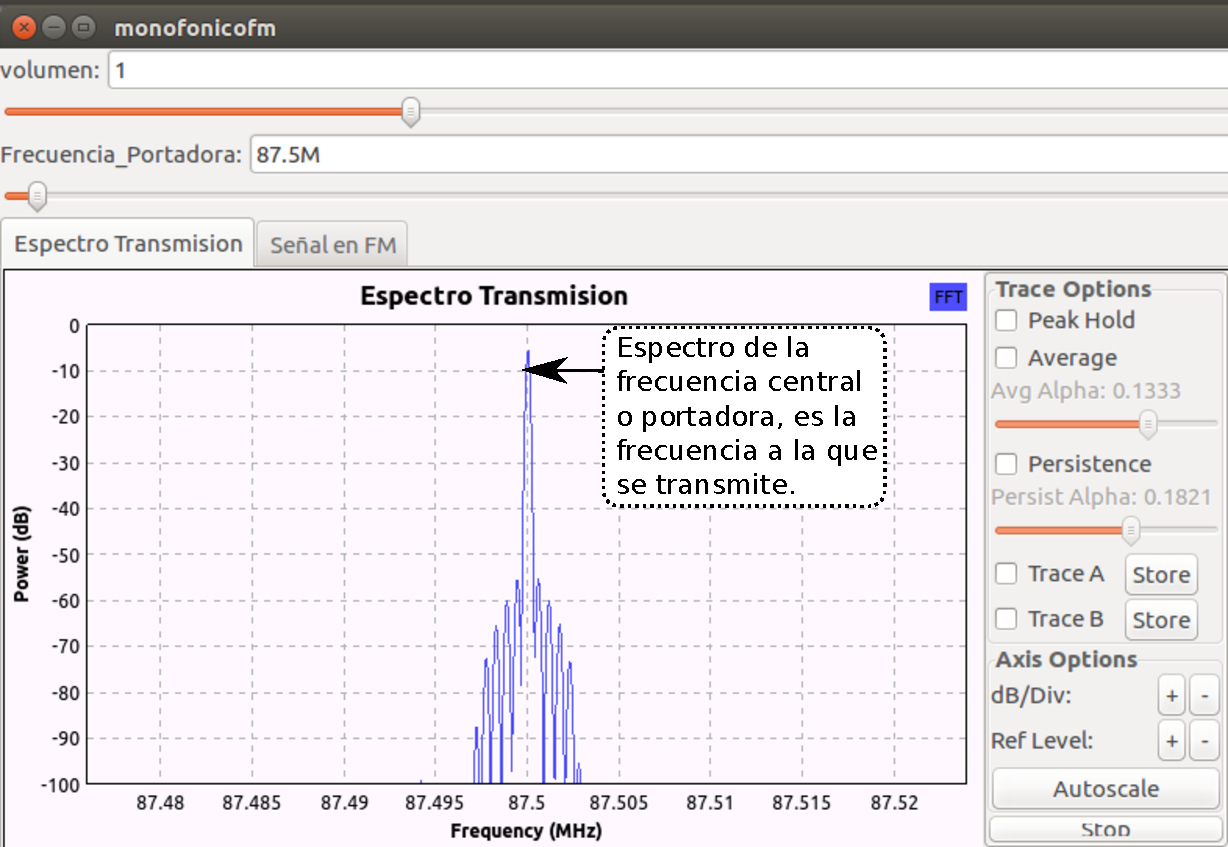
\includegraphics[width=\textwidth]{parte3/lab11/pdf/lab11_6.pdf}
\end{figure}

\end{frame}
%---------------------------------

\begin{frame}{Transmisor FM monofónico}

\begin{figure}[H]
\centering
\vspace{-3mm}
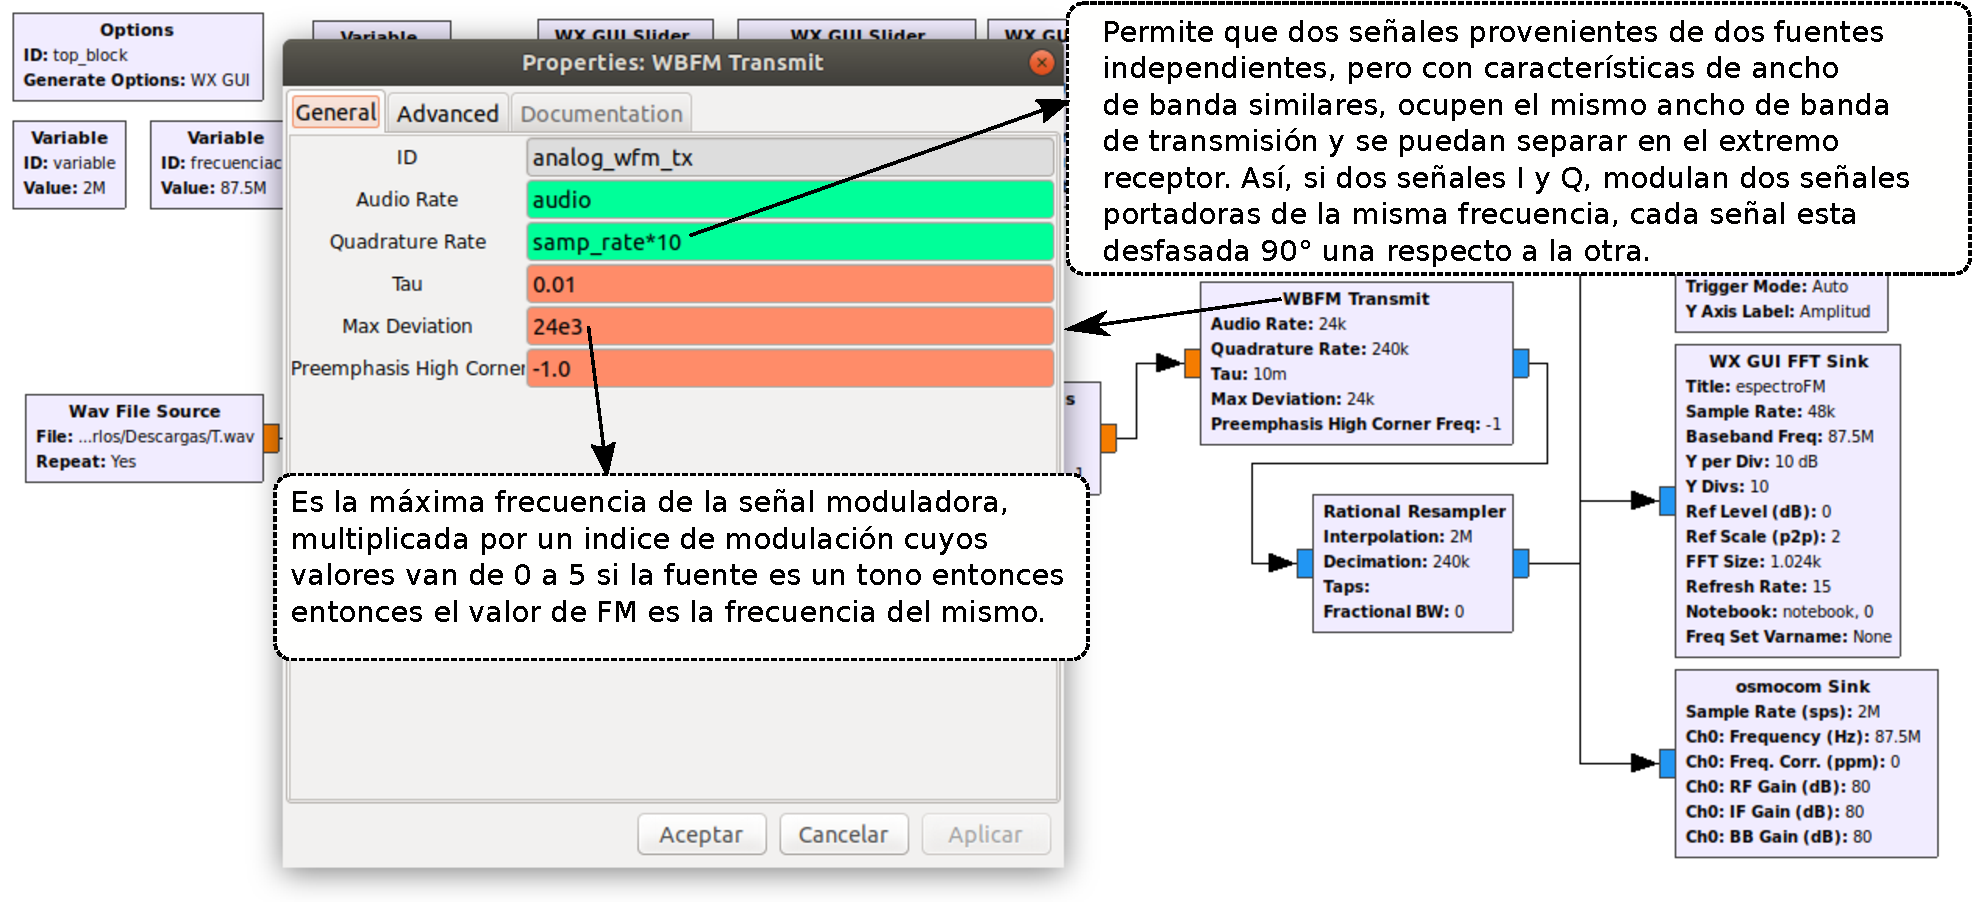
\includegraphics[width=\textwidth]{parte3/lab11/pdf/lab11_7.pdf}
\end{figure}

\end{frame}
%---------------------------------

\begin{frame}{Transmisor FM monofónico}

\begin{figure}[H]
\centering
\vspace{-3mm}
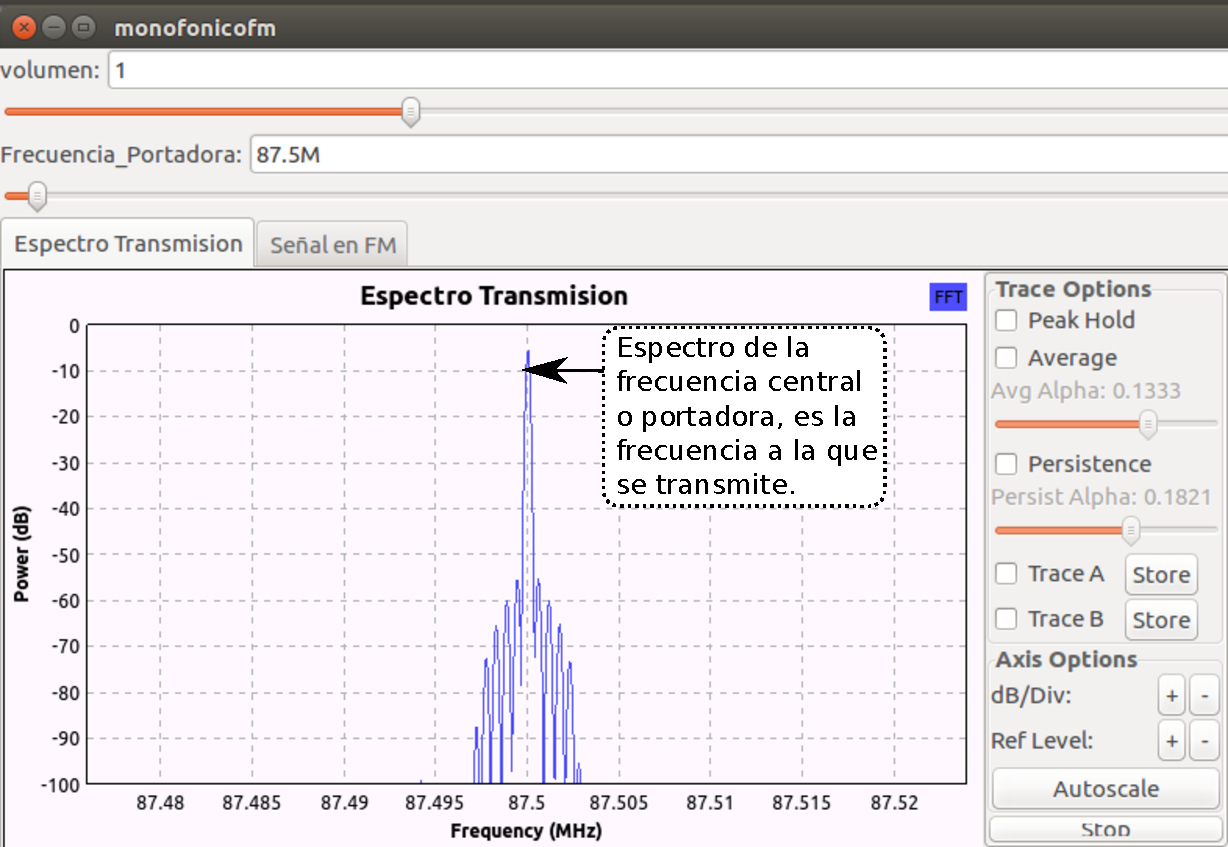
\includegraphics[width=.8\textwidth]{parte3/lab11/pdf/lab11_8.pdf}
\end{figure}

\end{frame}
%---------------------------------